% Created 2022-12-17 Sat 16:07
% Intended LaTeX compiler: pdflatex
\documentclass[a4paper,11pt]{article}
\usepackage[utf8]{inputenc}
\usepackage[T1]{fontenc}
\usepackage{graphicx}
\usepackage{longtable}
\usepackage{wrapfig}
\usepackage{rotating}
\usepackage[normalem]{ulem}
\usepackage{amsmath}
\usepackage{amssymb}
\usepackage{capt-of}
\usepackage{hyperref}
\usepackage[margin=1in]{geometry}
\usepackage{titlesec}
\usepackage{caption}
\usepackage{subcaption}
\usepackage{lipsum}
\author{Varghese Reji}
\date{}
\title{Classical and Quantum Optics\\\medskip
\large Assignment-2 Answers}
\hypersetup{
 pdfauthor={Varghese Reji},
 pdftitle={Classical and Quantum Optics},
 pdfkeywords={},
 pdfsubject={},
 pdfcreator={Emacs 28.2 (Org mode 9.5.5)}, 
 pdflang={English}}
\begin{document}

\maketitle

\section*{Problem 1}
\label{sec:orgce068e2}

A beam with a photon flux of 1000 photons s\textsuperscript{-1} is incident on a detector with a quantum efficiency of 20\%. If the time interval of the counter is set to 10s, calculate the average and standard deviation of the photocount number for the followin g scenarios:
\begin{description}
\item[{(a)}] the light has Poissonian statistics;
\item[{(b)}] the light has super-Poissonian statistics with \(\Delta\) n=2\texttimes{} \(\Delta\) n\textsubscript{Poisson} ;
\item[{(c)}] the light is in a photon number state.
\end{description}

\subsection*{Answer}
\label{sec:orga615958}
\(\phi\) = 1000/s, \(\eta\)=20\%, t=10s

\begin{description}
\item[{(a)}] \(\bar{n} = \frac{L \phi}{c}\)

But, \(L=ct \Rightarrow \bar{n} = t \phi\)

Then, \(\bar{n} = 10000\).\$

\(\Delta n = \sqrt{n} = 100\)

The photocount number is given by, $$(\Delta N)^2 = \eta^2(\Delta n)^2 + \eta(1-\eta) \bar{n}$$

\(\Rightarrow\), $$\Delta N = 44.721$$.

$$\bar{N} = \eta \bar{n} = 2000$$
\end{description}


\begin{description}
\item[{(b)}] Given \(\Delta n = 2\times \Delta n_{Poisson}\).
i.e., \(\Delta n = 89.442\)
\end{description}



We know that, for super poissonian statistics,

$$(\Delta n)^2 = \bar{n} + \bar{n}^2$$.

\(\Rightarrow\)

$$ \bar{n} + \bar{n}^2 = 4 \bar{n}_{Poiss}^2 = 8000$$

By solving this,

$$\bar{n} =88.944$$


$$\Delta N = 18.28, \bar{N} = 17.79$$

\begin{description}
\item[{(c)}] In phton number state, \(\Delta n=0\). That means, there is no variation from mean value. Then, \(\bar{n} = 10000\)
\end{description}

\(\Rightarrow\)
$$\bar{N} = 2000, \Delta N = 40$$

\section*{Problem 2}
\label{sec:org49829e5}
Calculate the values of g\textsuperscript{(2)}(0) for a monochromatic light wave with a square wave intensity modulation of \textpm{} 20\%.

\subsection*{Answer}
\label{sec:org01978a4}

$$g^(2)(0) = \frac{\langle I(t)^2\rangle }{\langle I(t)\rangle ^2}$$

Since the intensity modulation is A=0.2, let us write, $$I(t) = I_0(1+0.2\Theta(T/2))$$

\(\Theta\) is a square pulse.
$$\langle I(t)\rangle ^2 = I_0^2$$

$$\langle I(t)^2\rangle  = \frac{I_0^2}{T} \int_0^{T} (1+0.2\Theta(T/2)) ^2$$

Then,
\begin{equation*}
\begin{split}
g^{(2)}(0) & = \frac{1}{T} \int_0^T dt (1+0.2\Theta(T/2))^2 \\
 & = \frac{1}{T} \left[\int_0^Tdt+0.4\int_0^{T/2}dt+0.04\int_0^{T/2}dt\right] \\
& = 1+0.2+0.02\\
& = 1.22
\end{split}
\end{equation*}


Then, $$g^(2)(0) = 1.22$$


\section*{Problem 3}
\label{sec:org07a6ba4}
The 632.8 nm line of a neon discharge lamp is Doppler-broadened with a linewidth of 1.5GHz. Sketch the second-order correlation function g\textsuperscript{(2)}(\(\tau\)) for \(\tau\) in range 0-1 ns.

\subsection*{Answer}
\label{sec:org61e46ea}
The coherence time is given by the formula

$$\tau_c = \frac{\lambda^2}{c\delta \lambda}$$

Given, \(\Delta \nu = 1.5GHz\).

And, \(d\lambda = \frac{c}{\lambda^2} d\nu \Rightarrow \tau_c = \frac{1}{d\nu}\)

\(\therefore\)

$$\tau_c = 6.67e-10s = .667 ns$$

From Mark Fox,

$$g^{(2)}(\tau) = 1+\exp\left[-\pi\left(\frac{\tau}{\tau_c}\right)^2\right]$$

\begin{center}
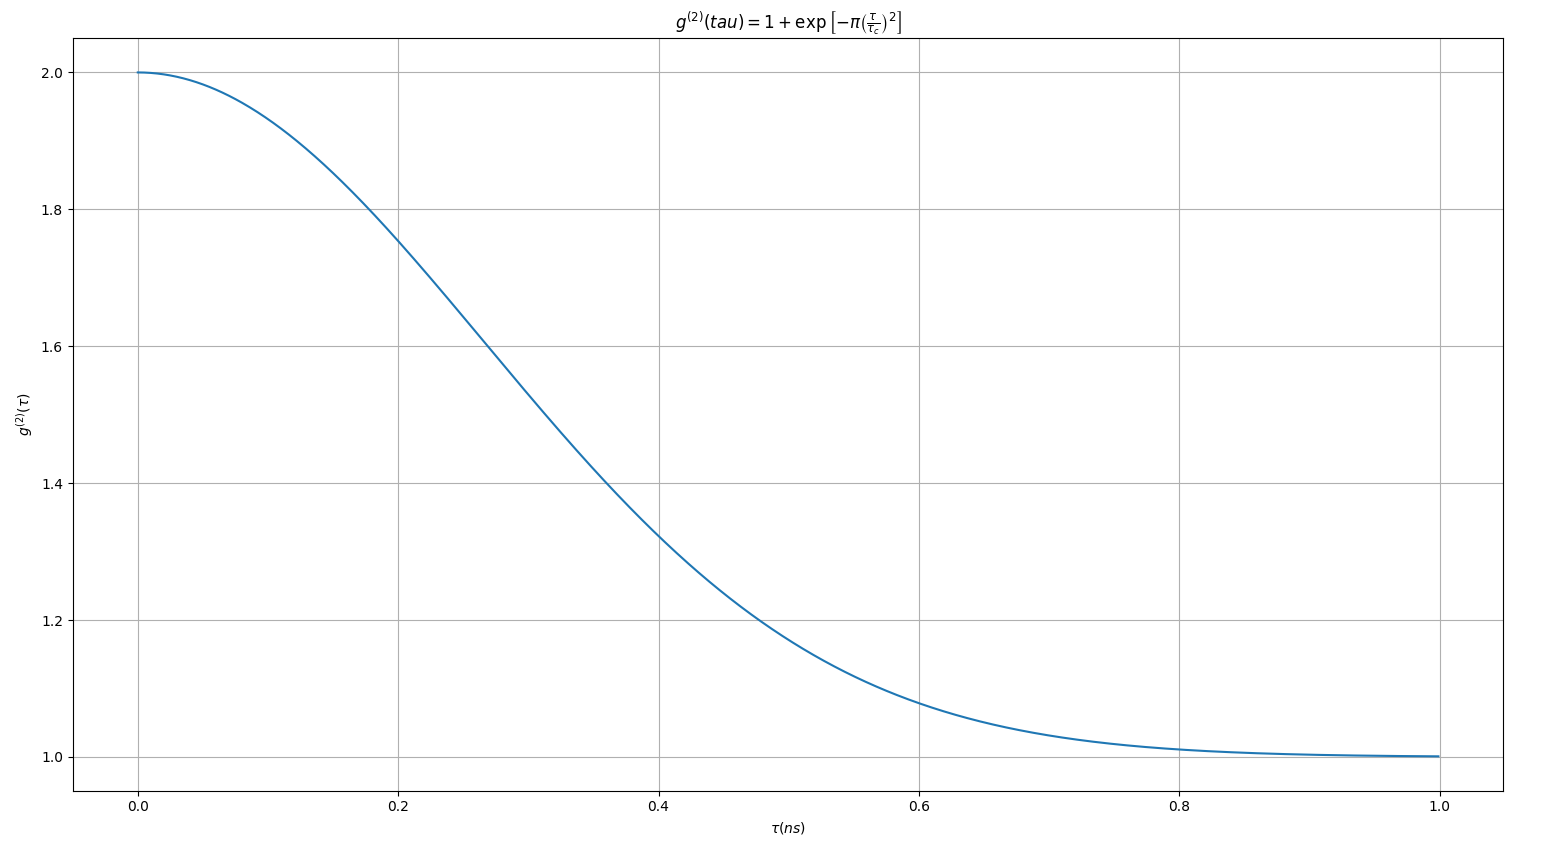
\includegraphics[width=.9\linewidth]{pr3_plot.png}
\end{center}



\section*{Problem 4}
\label{sec:org3b46d2f}
For the coherent states |\(\alpha \rangle\)  with \(\alpha\)=5, calculate
\begin{description}
\item[{(a)}] the mean photon number;
\item[{(b)}] the standard deviation in the photon number;
\item[{(c)}] the quantum uncertinity in the optical phase.
\end{description}

\subsection*{Answer}
\label{sec:org6415c01}
\begin{description}
\item[{(a)}] \(\alpha = 5\). Then, \(\bar{n} = |\alpha|^2 = 25\)

\item[{(b)}] \(\Delta n = |\alpha| = 5\)

\item[{(c)}] \(\Delta \phi = \frac{\text{uncertinity diameter}}{\alpha} = \frac{1/2}{5} = \frac{1}{10}\)
\end{description}
\section*{Problem 5}
\label{sec:org44d27ad}
A ruby laser operating at 693 nm emits pulses of energy 1mJ. Calculate the quantum uncertinity in the phase of the laser light.

\subsection*{Answer}
\label{sec:org26cdd62}

\(\lambda = 693nm, E=1mJ\).

Then, $$n = 3.486\times 10^{15}$$

n := 3.486e15

a := n\textsuperscript{0.5} =\(\rangle\)  59042357.6765

dp := 0.5 / a =\(\rangle\)  8.46849651126e-9

Then, $$\Delta \phi = \frac{\text{uncertinity diameter}}{\alpha}=\frac{1/2}{59042357.6765} = 8.468\times 10{-9}$$
\section*{Problem 6}
\label{sec:org4acf728}
For the coherent state |\(\alpha \rangle\)  with \(\alpha\)=|\(\alpha\)|e\textsuperscript{i\(\phi\)}, show that \(\langle \alpha|\hat{X}_1|\alpha\rangle =|\alpha|\cos\phi\) and \(\langle \alpha|\hat{X}_2|\alpha\rangle =|\alpha|\sin\phi\). Show further that \(\Delta X_1 = \Delta X_2 = \frac{1}{2}\).

\subsection*{Answer}
\label{sec:org737bc0c}
$$\hat{X}_1 = \frac{1}{2} (\hat{a}^\dag+\hat{a})~~~~~~\hat{X}_2 = \frac{i}{2} (\hat{a}^\dag-\hat{a})$$

$$\hat{a}|n\rangle = (n)^\frac{1}{2}|n-1\rangle~~~~~~\hat{a}^\dag|n\rangle = (n+1)^\frac{1}{2}|n+1\rangle$$
$$|\alpha\rangle = \exp\left(-\frac{|\alpha|^2}{2}\right) \sum_{n=0}^{\infty}\frac{\alpha^n}{(n!)^\frac{1}{2}}|n\rangle$$

\begin{equation*}
\begin{split}
\langle\alpha|\hat{X}_1|\alpha\rangle & =\frac{1}{2} \exp\left(-|\alpha|^2\right) \sum_{n=0}^{\infty}\frac{\alpha*^n}{(n!)^\frac{1}{2}}  \sum_{m=0}^{\infty}\frac{\alpha^m}{(m!)^\frac{1}{2}}\langle n|(\hat{a}^\dag+\hat{a}) |m\rangle \\
& = \frac{1}{2} \exp\left(-|\alpha|^2\right) \sum_{n=0}^{\infty}\frac{\alpha*^n}{(n!)^\frac{1}{2}}  \sum_{m=0}^{\infty}\frac{\alpha^m}{(m!)^\frac{1}{2}}\left[(m+1)^\frac{1}{2}\langle n|m+1\rangle+m^\frac{1}{2}\langle n |m-1\rangle\right] \\
& = \frac{1}{2} \exp\left(-|\alpha|^2\right) \sum_{n=0}^{\infty}\frac{\alpha*^n}{(n!)^\frac{1}{2}}  \sum_{m=0}^{\infty}\frac{\alpha^m}{(m!)^\frac{1}{2}}\left[(m+1)^\frac{1}{2}\delta_{n,m+1}+m^\frac{1}{2}\delta_{n,m-1}\right] \\
& = \exp\left(-|\alpha|^2\right) \sum_{n=0}^{\infty}\left[\frac{\alpha*^n}{(n!)^\frac{1}{2}}  \frac{\alpha^m}{(m!)^\frac{1}{2}}(m+1)^\frac{1}{2}\delta_{n,m+1}+\frac{\alpha*^n}{(n!)^\frac{1}{2}}  \frac{\alpha^m}{(m!)^\frac{1}{2}}m^\frac{1}{2}\delta_{n,m-1}\right] \\
& = \frac{1}{2} \exp\left(-|\alpha|^2\right) \sum_{n=0}^{\infty}\left[\frac{\alpha*^{m+1}}{((m+1)!)^\frac{1}{2}}  \frac{\alpha^m}{(m!)^\frac{1}{2}}(m+1)^\frac{1}{2}+\frac{\alpha^{m-1}}{((m-1)!)^\frac{1}{2}}  \frac{\alpha^m}{(m!)^\frac{1}{2}}m^\frac{1}{2}\right] \\
& = \frac{1}{2} \exp\left(-|\alpha|^2\right) \sum_{n=0}^{\infty}\left[\frac{\alpha*^{m+1}\alpha^m}{m!}  +\frac{\alpha^{m-1}\alpha^m}{((m-1)!)}\right] \\
& = \frac{1}{2} \exp\left(-|\alpha|^2\right) \sum_{n=0}^{\infty}\left[\alpha*\frac{\alpha^{2m}}{m!}  +\alpha\frac{\alpha^{2(m-1)}}{((m-1)!)}\right] \\
& = \frac{1}{2} \left[\alpha* +\alpha\right] \\
& = \frac{|\alpha|}{2}(e^{i\phi} + e^{-i\phi}) \\
& = |\alpha|\cos\phi
\end{split}
\end{equation*}


\begin{equation*}
\begin{split}
\langle\alpha|\hat{X}_1|\alpha\rangle & =\frac{1}{2} \exp\left(-|\alpha|^2\right) \sum_{n=0}^{\infty}\frac{\alpha*^n}{(n!)^\frac{1}{2}}  \sum_{m=0}^{\infty}\frac{\alpha^m}{(m!)^\frac{1}{2}}\langle n|(\hat{a}^\dag-\hat{a}) |m\rangle \\
& = i\frac{1}{2} \exp\left(-|\alpha|^2\right) \sum_{n=0}^{\infty}\frac{\alpha*^n}{(n!)^\frac{1}{2}}  \sum_{m=0}^{\infty}\frac{\alpha^m}{(m!)^\frac{1}{2}}\left[(m+1)^\frac{1}{2}\langle n|m+1\rangle-m^\frac{1}{2}\langle n |m-1\rangle\right] \\
& = i\frac{1}{2} \exp\left(-|\alpha|^2\right) \sum_{n=0}^{\infty}\frac{\alpha*^n}{(n!)^\frac{1}{2}}  \sum_{m=0}^{\infty}\frac{\alpha^m}{(m!)^\frac{1}{2}}\left[(m+1)^\frac{1}{2}\delta_{n,m+1}-m^\frac{1}{2}\delta_{n,m-1}\right] \\
& = i\exp\left(-|\alpha|^2\right) \sum_{n=0}^{\infty}\left[\frac{\alpha*^n}{(n!)^\frac{1}{2}}  \frac{\alpha^m}{(m!)^\frac{1}{2}}(m+1)^\frac{1}{2}\delta_{n,m+1}-\frac{\alpha*^n}{(n!)^\frac{1}{2}}  \frac{\alpha^m}{(m!)^\frac{1}{2}}m^\frac{1}{2}\delta_{n,m-1}\right] \\
& = i\frac{1}{2} \exp\left(-|\alpha|^2\right) \sum_{n=0}^{\infty}\left[\frac{\alpha*^{m+1}}{((m+1)!)^\frac{1}{2}}  \frac{\alpha^m}{(m!)^\frac{1}{2}}(m+1)^\frac{1}{2}-\frac{\alpha^{m-1}}{((m-1)!)^\frac{1}{2}}  \frac{\alpha^m}{(m!)^\frac{1}{2}}m^\frac{1}{2}\right] \\
& = i\frac{1}{2} \exp\left(-|\alpha|^2\right) \sum_{n=0}^{\infty}\left[\frac{\alpha*^{m+1}\alpha^m}{m!}  -\frac{\alpha^{m-1}\alpha^m}{((m-1)!)}\right] \\
& = i\frac{1}{2} \exp\left(-|\alpha|^2\right) \sum_{n=0}^{\infty}\left[\alpha*\frac{\alpha^{2m}}{m!}  -\alpha\frac{\alpha^{2(m-1)}}{((m-1)!)}\right] \\
& = i\frac{1}{2} \left[\alpha* -\alpha\right] \\
& = i\frac{|\alpha|}{2}(e^{-i\phi} - e^{i\phi}) \\
& = |\alpha|\sin\phi
\end{split}
\end{equation*}

$$\hat{X}_1^2 = \frac{1}{4} (\hat{a}^\dag+\hat{a})^2 = \frac{1}{4} (\hat{a}^\dag\hat{a}^\dag+\hat{a}\hat{a}+\hat{a}^\dag\hat{a}+\hat{a}\hat{a}^\dag) $$
$$\hat{X}_2^2 = \frac{-1}{4} (\hat{a}^\dag-\hat{a})^2 = \frac{1}{4} (-\hat{a}^\dag\hat{a}^\dag-\hat{a}\hat{a}+\hat{a}^\dag\hat{a}+\hat{a}\hat{a}^\dag) $$

Using the commutator \([\hat{a},\hat{a}^\dag] = 1, \hat{a}\hat{a}^\dag = 1+ \hat{a}^\dag\hat{a}\)

\(\Rightarrow\)

$$\hat{X}_1^2 = \frac{1}{4} (\hat{a}^\dag+\hat{a})^2 = \frac{1}{4} (\hat{a}^\dag\hat{a}^\dag+\hat{a}\hat{a}+2\hat{a}^\dag\hat{a}+1) $$
$$\hat{X}_2^2 = \frac{-1}{4} (\hat{a}^\dag-\hat{a})^2 = \frac{1}{4} (-\hat{a}^\dag\hat{a}^\dag-\hat{a}\hat{a}+2\hat{a}^\dag\hat{a}+1) $$


\begin{equation*}
\begin{split}
\langle\alpha|\hat{X}_1^2|\alpha\rangle & =\frac{1}{4} \exp\left(-|\alpha|^2\right) \sum_{n=0}^{\infty}\frac{\alpha*^n}{(n!)^\frac{1}{2}}  \sum_{m=0}^{\infty}\frac{\alpha^m}{(m!)^\frac{1}{2}}\langle n|(\hat{a}^\dag\hat{a}^\dag+\hat{a}\hat{a}+2\hat{a}^\dag\hat{a}+1) |m\rangle \\
\sum_{n=0}^{\infty}\frac{\alpha*^n}{(n!)^\frac{1}{2}}  & \sum_{m=0}^{\infty}\frac{\alpha^m}{(m!)^\frac{1}{2}}\langle n|m\rangle  = \sum_{m=0}^{\infty}\frac{|\alpha|^{2m}}{m!} = \exp\left(|\alpha|^2\right) \\
\sum_{n=0}^{\infty}\frac{\alpha*^n}{(n!)^\frac{1}{2}}  & \sum_{m=0}^{\infty}\frac{\alpha^m}{(m!)^\frac{1}{2}}\langle n|\hat{a}^\dag\hat{a}|m\rangle = \sum_{n=0}^{\infty}\frac{\alpha*^n}{(n!)^\frac{1}{2}}\sum_{m=0}^{\infty}\frac{\alpha^m}{(m!)^\frac{1}{2}}m\langle n|m\rangle \\
& = \sum_{m=1}^{\infty}\frac{|\alpha|^{2m}}{(m-1)!} = |\alpha|^2 \exp\left(|\alpha|^2\right)\\
\sum_{n=0}^{\infty}\frac{\alpha*^n}{(n!)^\frac{1}{2}}  & \sum_{m=0}^{\infty}\frac{\alpha^m}{(m!)^\frac{1}{2}}\langle n|\hat{a}\hat{a}|m\rangle = \sum_{n=0}^{\infty}\frac{\alpha*^n}{(n!)^\frac{1}{2}}   \sum_{m=0}^{\infty}\frac{\alpha^m}{(m!)^\frac{1}{2}}(m(m-1))^\frac{1}{2}\langle n|m-2\rangle \\
& = \sum_{n=0}^{\infty}\frac{\alpha*^n}{(n!)^\frac{1}{2}}  \sum_{m=0}^{\infty}\frac{\alpha^m}{(m!)^\frac{1}{2}}(m(m-1))^\frac{1}{2}\delta_{n, m-2} \\
& = \sum_{m=2}^{\infty}\frac{\alpha*^{m-2}\alpha^m}{((m-2)!)} \\
& = \alpha^2\sum_{m=2}^{\infty}\frac{|\alpha|^{2(m-2)}}{((m-2)!)} \\
& = \alpha^2 \exp\left(|\alpha|^2\right)\\
\sum_{n=0}^{\infty}\frac{\alpha*^n}{(n!)^\frac{1}{2}}  & \sum_{m=0}^{\infty}\frac{\alpha^m}{(m!)^\frac{1}{2}}\langle n|\hat{a}^\dag\hat{a}^\dag|m\rangle = \sum_{n=0}^{\infty}\frac{\alpha*^n}{(n!)^\frac{1}{2}}   \sum_{m=0}^{\infty}\frac{\alpha^m}{(m!)^\frac{1}{2}}((m+1)(m+2))^\frac{1}{2}\langle n|m+2\rangle \\
& = \sum_{n=0}^{\infty}\frac{\alpha*^n}{(n!)^\frac{1}{2}}   \sum_{m=0}^{\infty}\frac{\alpha^m}{(m!)^\frac{1}{2}}((m+1)(m+2))^\frac{1}{2}\delta_{n, m+2} \\
& = \sum_{n=0}^{\infty}\frac{\alpha*^n}{(n!)^\frac{1}{2}}   \sum_{m=0}^{\infty}\frac{\alpha^m}{(m!)^\frac{1}{2}}((m+1)(m+2))^\frac{1}{2}\delta_{n-2,m} \\
& = \sum_{n=2}^{\infty}\frac{\alpha*^n}{((n-2)!)^\frac{1}{2}}   \frac{\alpha^{n-2}}{((n-2)!)^\frac{1}{2}} \\
& = \alpha*^2\sum_{n=2}^{\infty}\frac{|\alpha|^{2n-4}}{((n-2)!)} \\
& = \alpha*^2 \exp\left(|\alpha|^2\right)\\
\end{split}
\end{equation*}

\begin{equation*}
\begin{split}
\langle\alpha|\hat{X}_1^2|\alpha\rangle & = \frac{1}{4} (\alpha*^2+\alpha^2+2|\alpha|^2 +1) \\
& = \frac{1}{4} (\alpha*^2+\alpha^2+2\alpha * \alpha +1) \\
& = \frac{1}{4} ((\alpha+\alpha*)^2 +1) \\
& = \alpha^2\cos^2\phi + \frac{1}{4}
\end{split}
\end{equation*}

Similerly,

\begin{equation*}
\begin{split}
\langle\alpha|\hat{X}_2^2|\alpha\rangle & = \frac{1}{4} (-\alpha*^2-\alpha^2+2|\alpha|^2 +1) \\
& = \frac{1}{4} (-\alpha*^2-\alpha^2+2\alpha * \alpha +1) \\
& = \frac{1}{4} (-(\alpha-\alpha*)^2 +1) \\
& = \alpha^2\sin^2\phi + \frac{1}{4}
\end{split}
\end{equation*}

Then,

$$\Delta \hat{X}_1^2 = \alpha^2\cos^2\phi + \frac{1}{4} - \alpha^2\cos^2\phi = \frac{1}{4}$$
$$\Delta \hat{X}_1^2 = \alpha^2\sin^2\phi + \frac{1}{4} - \alpha^2\sin^2\phi = \frac{1}{4}$$

Then, $$\Delta\hat{X}_1 = \Delta\hat{X}_2 = \frac{1}{2}$$
\section*{Problem 7}
\label{sec:org59a5f45}
Prove that for two coherent states |\(\alpha \rangle\)  and |\(\beta \rangle\) ,
$$|\langle \alpha|\beta\rangle |^2=\exp(-|\alpha-\beta|^2)$$

\subsection*{Answer}
\label{sec:org5949911}

Since both \(|\alpha\rangle\) and \(|\beta\rangle\) are coherent states,

$$|\alpha\rangle = \exp\left(-\frac{|\alpha|^2}{2}\right) \sum_{n=0}^{\infty}\frac{\alpha^n}{(n!)^\frac{1}{2}}|n\rangle ~~~~~~|\beta\rangle = \exp\left(-\frac{|\beta|^2}{2}\right) \sum_{m=0}^{\infty}\frac{\beta^m}{(m!)^\frac{1}{2}}|m\rangle$$

\begin{equation*}
\begin{split}
\langle \alpha |\beta \rangle & = \exp\left(-\frac{|\alpha|^2+|\beta|^2}{2}\right) \sum_{n=0}^{\infty}\sum_{m=0}^{\infty}\frac{\alpha^n\beta^m}{(n!)^\frac{1}{2}(m!)^\frac{1}{2}}\langle n | m\rangle \\
& = \exp\left(-\frac{|\alpha|^2+|\beta|^2}{2}\right) \sum_{n=0}^{\infty}\sum_{m=0}^{\infty}\frac{\alpha^n\beta^m}{(n!)^\frac{1}{2}(m!)^\frac{1}{2}}\delta_{nm} \\
& = \exp\left(-\frac{|\alpha|^2+|\beta|^2}{2}\right) \sum_{n=0}^{\infty}\sum_{n=0}^{\infty}\frac{(\alpha*\beta)^n}{(n!)} \\
& = \exp\left(-\frac{|\alpha|^2+|\beta|^2}{2}\right) \exp\left(\alpha*\beta\right)\\
& = \exp\left(-\frac{|\alpha|^2-2\alpha*\beta+|\beta|^2}{2}\right)\\
& = \exp\left(-\frac{|\alpha-\beta|^2}{2}\right)\\
\end{split}
\end{equation*}

Then, while taking the square of this,

$$|\langle \alpha|\beta\rangle |^2=\exp(-|\alpha-\beta|^2)$$
\end{document}